\documentclass[10pt,aspectratio=169]{beamer}

\usetheme[progressbar=foot]{metropolis}
\AtBeginSection{}

\usepackage{appendixnumberbeamer}
\usepackage{booktabs}
\usepackage[scale=2]{ccicons}
\usepackage{tabularx}
\usepackage{tikz}
\usetikzlibrary{arrows.meta,positioning,shapes.geometric,fit}
\usepackage{xspace}
\newcommand{\themename}{\textbf{\textsc{metropolis}}\xspace}
\usepackage{comment}
\usepackage{caption}
\usepackage[
  backend=biber,
  style=authoryear
]{biblatex}

\setbeamertemplate{bibliography item}{}
\addbibresource{bibliography.bib}

\usepackage{graphicx}
\usepackage{siunitx}



%................................................................................
% COLORS

\definecolor{ukudlaBlue}{RGB}{41, 60, 135}
\definecolor{ukudlaLightBlue}{RGB}{212, 216, 231}
\definecolor{ukudlaRed}{RGB}{164, 28, 34}
\definecolor{ukudlaLightRed}{RGB}{236, 209, 210}
\definecolor{ukudlaGreen}{RGB}{59, 139, 71}
\definecolor{ukudlaLightGreen}{RGB}{215, 231, 218}
\definecolor{ukudlaYellow}{RGB}{239, 198, 44}
\definecolor{ukudlaLightYellow}{RGB}{251, 243, 212}
\definecolor{white}{RGB}{255, 255, 255}
\definecolor{black}{RGB}{0, 0, 0}

\setbeamercolor{palette primary}{fg=white, bg=ukudlaGreen}
\setbeamercolor{progress bar}{fg=ukudlaRed, bg=ukudlaYellow}
\setbeamercolor{title separator}{fg=ukudlaRed, bg=ukudlaYellow}
\setbeamercolor{progress bar in head/foot}{fg=ukudlaRed, bg=ukudlaYellow}
\setbeamercolor{progress bar in section page}{fg=ukudlaRed, bg=ukudlaYellow}
\setbeamercolor{background canvas}{bg=white}

\setbeamercolor{block body}{bg=ukudlaLightGreen,fg=black}



%................................................................................
% PRESENTATION INFORMATION

\title{UKUDLA Data Science Certificate}
\subtitle{Reproducible Environments using \texttt{renv} \& Docker}
\author{Markus Mößler}
\institute{University of Hohenheim}



%................................................................................
% CUSTOM FOOTER

\makeatletter
\setbeamertemplate{progress bar in head/foot}{%
  \tikzset{metropolis@progressbar@foreground/.style={fill=ukudlaGreen}}%
  \tikzset{metropolis@progressbar@background/.style={fill=ukudlaLightGreen}}%

  \begin{tikzpicture}[overlay, x=\paperwidth, y=1cm]
    \fill[metropolis@progressbar@background]
      (0,0) rectangle (1,0.10);
    \fill[metropolis@progressbar@foreground]
      (0,0) rectangle
      ({\insertframenumber/\inserttotalframenumber},0.10);
    \node[anchor=south west, yshift=0.25cm, xshift=0.2cm]
      at (0,0)
      {\includegraphics[height=0.75cm]{./logos/UKUDLA_logo_03_white_bg.pdf}};
    % current section
    \ifnum\value{section}>0
      \node[
        anchor=south east,
        yshift=0.22cm,
        xshift=-0.60cm,
        fill=ukudlaLightGreen,
        rounded corners=2pt,
        inner xsep=6pt,
        inner ysep=3pt,
        font=\scriptsize\bfseries,
        text=ukudlaRed
      ] at (1,0) {
        \insertsectionhead
      };
    \fi

  \end{tikzpicture}%
}
\makeatother



%................................................................................
% CUSTOM TITLE PAGE

\makeatletter
\setbeamertemplate{title page}{
  \begin{beamercolorbox}[sep=8pt, center, wd=\paperwidth, ht=0.5\paperheight]{title page top}
    \begin{minipage}[c]{1.00\textwidth}
      \raggedleft
      \includegraphics[height=1.00cm]{./logos/ukudla_universities.pdf}
      \vspace*{0.2cm}
    \end{minipage}
    \begin{beamercolorbox}[wd=0.9\paperwidth, sep=12pt, left]{top box}
      {\usebeamerfont{title}\usebeamercolor[fg]{title}\inserttitle\par}
      \vskip0.1cm
      {\usebeamerfont{subtitle}\usebeamercolor[fg]{subtitle}\insertsubtitle\par}
    \end{beamercolorbox}
  \end{beamercolorbox}
  \begin{beamercolorbox}[sep=8pt, center, wd=\paperwidth, ht=0.5\paperheight]{title page bottom}
    \begin{beamercolorbox}[wd=0.9\paperwidth, sep=12pt, left]{bottom box}
      \hbox{%
        \hspace*{1em}
        \begin{minipage}[c]{0.40\textwidth}
          \vskip1.0cm
          {\usebeamerfont{author}\usebeamercolor[fg]{author}\insertauthor\par}
          \vskip0.1cm
          {\usebeamerfont{institute}\usebeamercolor[fg]{institute}\insertinstitute\par}
        \end{minipage}%
        \hspace*{1.5cm}
        \begin{minipage}[c]{1.00\textwidth}
          \includegraphics[height=2.0cm]{./logos/UKUDLA_logo_05.pdf}
        \end{minipage}%
      }
    \end{beamercolorbox}
    \begin{minipage}[r]{1.00\textwidth}
      \centering
      \includegraphics[width=1.00\textwidth]{./logos/ukudla_sponsors.pdf}
    \end{minipage}
  \end{beamercolorbox}
}
\makeatother

\setbeamercolor{title page top}{bg=white}
\setbeamercolor{top box}{bg=ukudlaGreen}
\setbeamercolor{title page bottom}{bg=white}
\setbeamercolor{bottom box}{bg=ukudlaLightGreen}
\setbeamercolor{title}{fg=white}
\setbeamercolor{subtitle}{fg=white}
\setbeamercolor{author}{fg=black}
\setbeamercolor{institute}{fg=black}
\setbeamercolor{date}{fg=black}



%................................................................................
% DOCUMENT

\begin{document}

\maketitle

%--------------------------------------------------
{
\setbeamertemplate{frame numbering}[none]

\begin{frame}[noframenumbering]{Table of contents}

  \small
  \setbeamertemplate{section in toc}[sections numbered]
  \tableofcontents[hideallsubsections]

\end{frame}
}
%--------------------------------------------------


\section{Motivation}


%--------------------------------------------------
% CONTENT SLIDE 1/10
\begin{frame}[fragile]{The reproducibility question}

\small

\begin{columns}[T]

\column{0.47\textwidth}

\textbf{Can another learner}

\begin{itemize}
  \item run the analysis scripts?
  \item obtain the required packages?
  \item reproduce the same results?
  \item recreate the analysis next year?
\end{itemize}

\column{0.47\textwidth}

\textbf{Environments can differ}

\begin{verbatim}
Learner A       Learner B
R 4.3.3         R 4.5.0
dplyr 1.1.4     dplyr 1.2.x
Ubuntu          Windows
\end{verbatim}

\end{columns}

\vspace{0.25cm}

\begin{beamercolorbox}[rounded=true,sep=9pt]{block body}
Sharing code is necessary, but code alone does not describe the computational conditions under which it ran. ``Works for me'' is not yet a reproducibility strategy.
\end{beamercolorbox}

\end{frame}
%--------------------------------------------------


%--------------------------------------------------
% CONTENT SLIDE 2/10
\begin{frame}{A computational environment has several layers}

\small

\centering

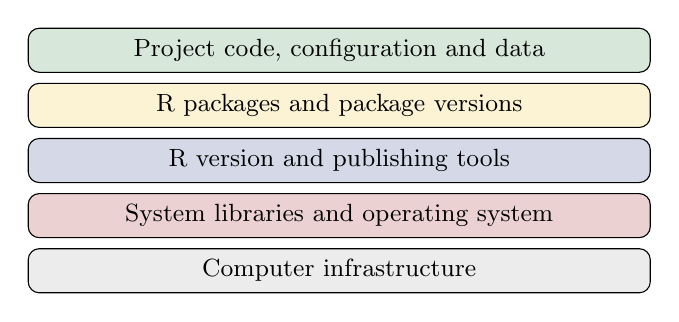
\begin{tikzpicture}[
  layer/.style={
    draw,
    rounded corners,
    minimum width=7.9cm,
    minimum height=0.56cm,
    align=center,
    font=\small
  }
]
  \node[layer,fill=ukudlaLightGreen] (project) at (0,2.05)
    {Project code, configuration and data};
  \node[layer,fill=ukudlaLightYellow] (packages) at (0,1.35)
    {R packages and package versions};
  \node[layer,fill=ukudlaLightBlue] (language) at (0,0.65)
    {R version and publishing tools};
  \node[layer,fill=ukudlaLightRed] (system) at (0,-0.05)
    {System libraries and operating system};
  \node[layer,fill=gray!15] (hardware) at (0,-0.75)
    {Computer infrastructure};
\end{tikzpicture}

\vspace{0.25cm}

\begin{columns}[T]

\column{0.31\textwidth}
\centering
\textbf{Isolation}\\
\scriptsize Keep project dependencies separate.

\column{0.31\textwidth}
\centering
\textbf{Portability}\\
\scriptsize Move work between computers.

\column{0.31\textwidth}
\centering
\textbf{Reproducibility}\\
\scriptsize Recreate recorded conditions.

\end{columns}

\end{frame}
%--------------------------------------------------


\section{Concepts}


%--------------------------------------------------
% CONTENT SLIDE 3/10
\begin{frame}{What does \texttt{renv} manage?}

\small

\begin{columns}[T]

\column{0.51\textwidth}

\textbf{\texttt{renv} provides}

\begin{itemize}
  \item a project-local R package library;
  \item isolation from other projects;
  \item a record of package versions and sources; and
  \item tools to restore that state.
\end{itemize}

\column{0.47\textwidth}

\textbf{\texttt{renv} does not manage}

\begin{itemize}
  \item the complete operating system;
  \item all system libraries;
  \item hardware or external services; or
  \item the research workflow itself.
\end{itemize}

\end{columns}

\vspace{0.25cm}

\begin{beamercolorbox}[rounded=true,sep=8pt]{block body}
\texttt{renv.lock} is a machine-readable description of the project's R
package environment and belongs in version control.
\end{beamercolorbox}

\end{frame}
%--------------------------------------------------


%--------------------------------------------------
% CONTENT SLIDE 4/10
\begin{frame}{The \texttt{renv} workflow}

\centering

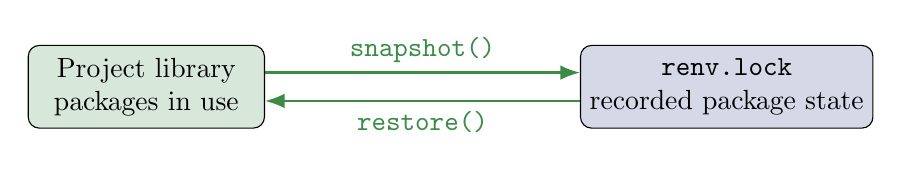
\begin{tikzpicture}[
  state/.style={
    draw,
    rounded corners,
    minimum height=1.05cm,
    minimum width=3.0cm,
    align=center
  },
  arrow/.style={-{Latex[length=2.5mm]},thick,ukudlaGreen}
]
  \node[state,fill=ukudlaLightGreen] (library)
    {Project library\\packages in use};
  \node[state,fill=ukudlaLightBlue, right=4.0cm of library] (lock)
    {\texttt{renv.lock}\\recorded package state};

  \draw[arrow] ([yshift=0.18cm]library.east) --
    node[above]{\texttt{snapshot()}} ([yshift=0.18cm]lock.west);
  \draw[arrow] ([yshift=-0.18cm]lock.west) --
    node[below]{\texttt{restore()}} ([yshift=-0.18cm]library.east);
\end{tikzpicture}

\vspace{0.50cm}

\small

\begin{itemize}
  \item \texttt{snapshot()} updates the lockfile from the project library.
  \item \texttt{restore()} recreates the project library from the lockfile.
  \item Review lockfile changes before committing them.
  \item A shared project can be initialized once and restored by collaborators.
\end{itemize}

\end{frame}
%--------------------------------------------------


%--------------------------------------------------
% CONTENT SLIDE 5/10
\begin{frame}{What does a container add?}

\small

\begin{columns}[T]

\column{0.49\textwidth}

\textbf{A container packages}

\begin{itemize}
  \item an operating-system user space;
  \item system libraries and tools;
  \item R and publishing tools;
  \item project dependencies; and
  \item a default working context.
\end{itemize}

\column{0.47\textwidth}

\textbf{A container shares}

\begin{itemize}
  \item the host computer's kernel;
  \item host hardware and resources;
  \item explicitly mounted files; and
  \item configured network access.
\end{itemize}

\end{columns}

\vspace{0.25cm}

\begin{beamercolorbox}[rounded=true,sep=8pt]{block body}
Containers provide stronger environment isolation than a project package library, but are lighter than a complete virtual machine.
\end{beamercolorbox}

\end{frame}
%--------------------------------------------------


%--------------------------------------------------
% CONTENT SLIDE 6/10
\begin{frame}{Dockerfile, image and container}

\centering

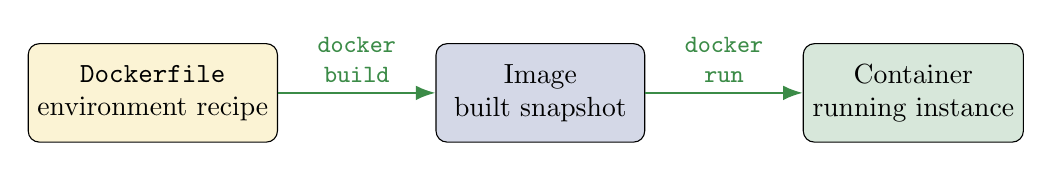
\begin{tikzpicture}[
  state/.style={
    draw,
    rounded corners,
    minimum height=1.25cm,
    minimum width=2.65cm,
    align=center
  },
  arrow/.style={-{Latex[length=2.5mm]},thick,ukudlaGreen},
  command/.style={font=\small\ttfamily}
]
  \node[state,fill=ukudlaLightYellow] (dockerfile)
    {\texttt{Dockerfile}\\environment recipe};
  \node[state,fill=ukudlaLightBlue, right=2.0cm of dockerfile] (image)
    {Image\\built snapshot};
  \node[state,fill=ukudlaLightGreen, right=2.0cm of image] (container)
    {Container\\running instance};

  \draw[arrow] (dockerfile) --
    node[above,command,align=center]{docker\\build} (image);
  \draw[arrow] (image) --
    node[above,command,align=center]{docker\\run} (container);
\end{tikzpicture}

\vspace{0.50cm}

\small

\begin{itemize}
  \item The Dockerfile describes how to construct an image.
  \item The image is an immutable snapshot that can be used repeatedly.
  \item Each container is a running instance created from that image.
  \item Rebuild after changing the Dockerfile or copied source code.
\end{itemize}

\end{frame}
%--------------------------------------------------


%--------------------------------------------------
\section{Application}
% CONTENT SLIDE 7/10

\begin{frame}{Containers are disposable; results must persist}

\small

\centering

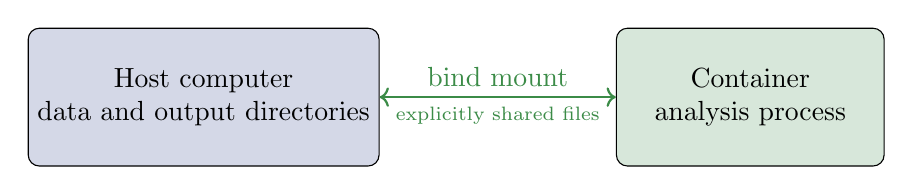
\begin{tikzpicture}[
  box/.style={
    draw,
    rounded corners,
    minimum width=3.4cm,
    minimum height=1.75cm,
    align=center
  },
  arrow/.style={<->,thick,ukudlaGreen}
]
  \node[box,fill=ukudlaLightBlue] (host)
    {Host computer\\data and output directories};
  \node[box,fill=ukudlaLightGreen, right=3.0cm of host] (container)
    {Container\\analysis process};
  \draw[arrow] (host) --
    node[above]{bind mount}
    node[below,font=\scriptsize]{explicitly shared files}
    (container);
\end{tikzpicture}

\vspace{0.50cm}

\raggedright

\begin{itemize}
  \item A container's writable layer normally disappears with the container.
  \item Bind mounts expose selected host directories inside the container.
  \item Inputs can be read and outputs written back to the host.
  \item Mount only what the analysis needs.
\end{itemize}

\end{frame}
%--------------------------------------------------


%--------------------------------------------------
% CONTENT SLIDE 8/10
\begin{frame}{Two tools manage different layers}

\small

\centering

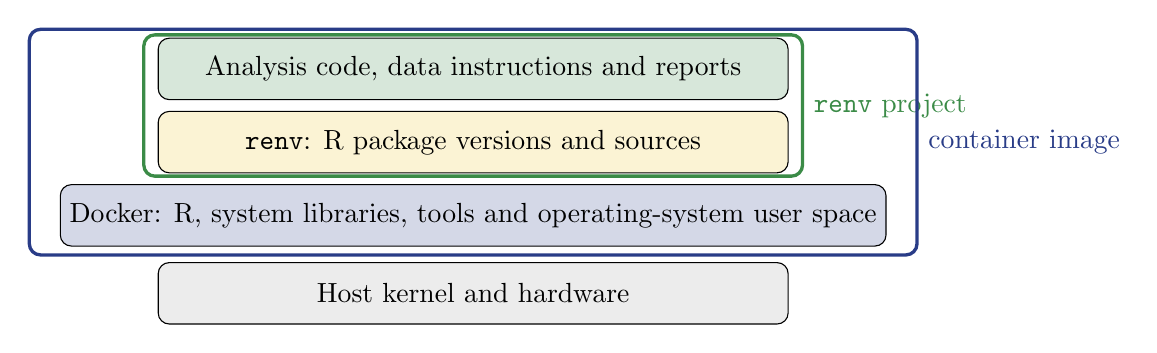
\begin{tikzpicture}[
  layer/.style={
    draw,
    rounded corners,
    minimum height=0.78cm,
    align=center
  }
]
  \node[layer,fill=ukudlaLightGreen,minimum width=8.0cm] (project) at (0,1.75)
    {Analysis code, data instructions and reports};
  \node[layer,fill=ukudlaLightYellow,minimum width=8.0cm] (renv) at (0,0.82)
    {\texttt{renv}: R package versions and sources};
  \node[layer,fill=ukudlaLightBlue,minimum width=8.0cm] (docker) at (0,-0.11)
    {Docker: R, system libraries, tools and operating-system user space};
  \node[layer,fill=gray!15,minimum width=8.0cm] (host) at (0,-1.10)
    {Host kernel and hardware};

  \node[
    draw=ukudlaGreen,
    very thick,
    rounded corners,
    fit=(project)(renv),
    inner xsep=5pt,
    inner ysep=1pt,
    label={[text=ukudlaGreen]right:\texttt{renv} project}
  ] {};

  \node[
    draw=ukudlaBlue,
    very thick,
    rounded corners,
    fit=(project)(renv)(docker),
    inner xsep=11pt,
    inner ysep=3pt,
    label={[text=ukudlaBlue]right:container image}
  ] {};
\end{tikzpicture}

\vspace{0.25cm}

\begin{beamercolorbox}[rounded=true,sep=8pt]{block body}
\texttt{renv} records the R package layer. Docker records a broader execution environment. Together they provide complementary reproducibility information.
\end{beamercolorbox}

\end{frame}
%--------------------------------------------------


%--------------------------------------------------
% CONTENT SLIDE 9/10
\begin{frame}{Run one analysis reproducibly across contexts}

\small

\begin{tabularx}{\textwidth}{@{}lXX@{}}
\toprule
\textbf{Method} & \textbf{Environment} & \textbf{Typical use} \\
\midrule
Local batch &
Host R with restored \texttt{renv} library &
Run the complete workflow \\
Local interactive &
RStudio or terminal R with \texttt{renv} &
Develop and inspect \\
Docker batch &
Image in a temporary container &
Run a consistent environment \\
Docker interactive &
Shell or R inside the container &
Inspect the container context \\
\bottomrule
\end{tabularx}

\vspace{0.30cm}

\centering

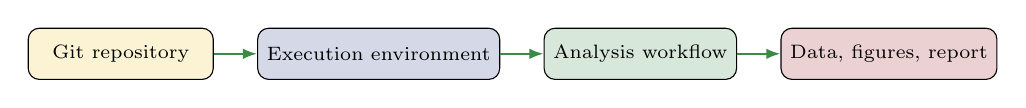
\begin{tikzpicture}[
  workflowstep/.style={
    draw,
    rounded corners,
    minimum width=2.35cm,
    minimum height=0.65cm,
    align=center,
    font=\scriptsize
  },
  arrow/.style={-{Latex[length=1.8mm]},thick,ukudlaGreen}
]
  \node[workflowstep,fill=ukudlaLightYellow] (repo)
    {Git repository};
  \node[workflowstep,fill=ukudlaLightBlue,right=0.55cm of repo] (environment)
    {Execution environment};
  \node[workflowstep,fill=ukudlaLightGreen,right=0.55cm of environment] (workflow)
    {Analysis workflow};
  \node[workflowstep,fill=ukudlaLightRed,right=0.55cm of workflow] (outputs)
    {Data, figures, report};
  \draw[arrow] (repo) -- (environment);
  \draw[arrow] (environment) -- (workflow);
  \draw[arrow] (workflow) -- (outputs);
\end{tikzpicture}

\end{frame}
%--------------------------------------------------


\section{Key Message}


%--------------------------------------------------
% CONTENT SLIDE 10/10
\begin{frame}{Key message: record every relevant environment layer}

\small

\begin{columns}[T]

\column{0.47\textwidth}

\textbf{Environment tools can help recreate}

\begin{itemize}
  \item package versions;
  \item language and system tools;
  \item execution commands; and
  \item a consistent working context.
\end{itemize}

\column{0.49\textwidth}

\textbf{They cannot guarantee}

\begin{itemize}
  \item correct data or code;
  \item valid scientific assumptions;
  \item permanent external sources; or
  \item responsible interpretation.
\end{itemize}

\end{columns}

\vspace{0.25cm}

\begin{beamercolorbox}[rounded=true,sep=8pt]{block body}
\texttt{renv} records R packages; Docker records a broader environment. Together with Git, documented data, and a reproducible workflow, they make an analysis easier to recreate and inspect.
\end{beamercolorbox}

\vspace{0.10cm}

% \centering
% \textcolor{ukudlaRed}{Reproducible does not automatically mean correct.}

\small
\centering

Detailed setup, repository, workflow, and troubleshooting instructions are provided in the learning-module guides.

\end{frame}
%--------------------------------------------------


%--------------------------------------------------
\begin{frame}[plain,noframenumbering]{Supported by}

  South African government and the National Research Foundation

  \begin{flushleft}
    \includegraphics[trim=0cm 0cm 0cm 0cm, clip, width=0.50\textwidth]{./logos/ukudla_south_african_sponsors.pdf}
  \end{flushleft}

  German government and the German Academic Exchange Service

  \begin{flushleft}
    \includegraphics[trim=0cm 0cm 0cm 0cm, clip, width=1.00\textwidth]{./logos/ukudla_german_sponsors.pdf}
  \end{flushleft}

\end{frame}
%--------------------------------------------------

\end{document}
